\documentclass[14 pt, fleqn, pstricks]{extarticle}

	\usepackage[frenchb]{babel}
	\usepackage[utf8]{inputenc}  
	\usepackage[T1]{fontenc}
	\usepackage{amssymb}
	\usepackage[mathscr]{euscript}
	\usepackage{stmaryrd}
	\usepackage{amsmath}
	\usepackage{tikz}
	\usepackage[all,cmtip]{xy}
	\usepackage{amsthm}
	\usepackage{varioref}
	\usepackage{geometry}
	\usepackage{tabularx}
	\geometry{a4paper}
	\usepackage{lmodern}
	\usepackage{hyperref}
	\usepackage{array}
	 \usepackage{fancyhdr}
	 \usepackage{pstricks,pst-plot,pst-tree,pstricks-add}
\usepackage{pst-eucl}% permet de faire des dessins de géométrie simplement
\usepackage{pst-text}
\usepackage{pst-node,pst-all}
\usepackage{pst-func,pst-math,pst-bspline,pst-3dplot}  %%% POUR LE BAC %%%
	 \usepackage{float}\usepackage{setspace}
\setlength{\mathindent}{1cm}
\renewcommand{\theenumi}{\alph{enumi})}
	\pagestyle{fancy}
	\theoremstyle{plain}
	\fancyfoot[C]{} 
	\fancyhead[L]{}
	\fancyhead[R]{}\geometry{
 a4paper,
 total={170mm,257mm}
 }
	
	
	\title{Exercices de calcul}
	\date{}
	\begin{document}
	 


\subsection*{Exercice 1 (6 points) }	 
	 Résoudre les équations suivantes : 
	 \begin{enumerate}
	 \item $ 2 x + 7 = 23$
	 \item $ 9 x + 2 = 3 x + 26$
	 \item $ (x-4)(x+2) = 0$
	 \item $(x+2)^2 - 1 = 0$
	 \end{enumerate}
\subsection*{Exercice 2 (7 points) }	
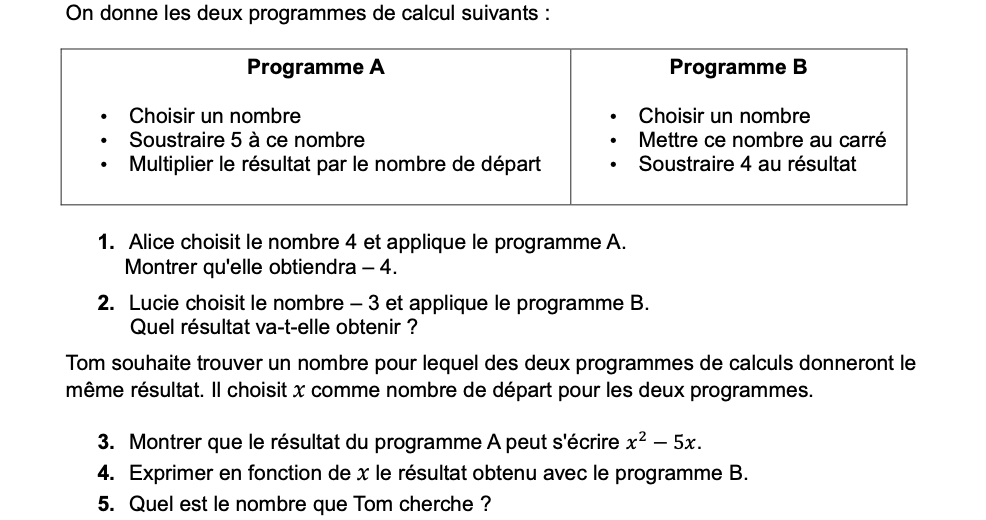
\includegraphics[width = 19 cm]{ex2} 
\subsection*{Exercice 3 (7 points) }	 
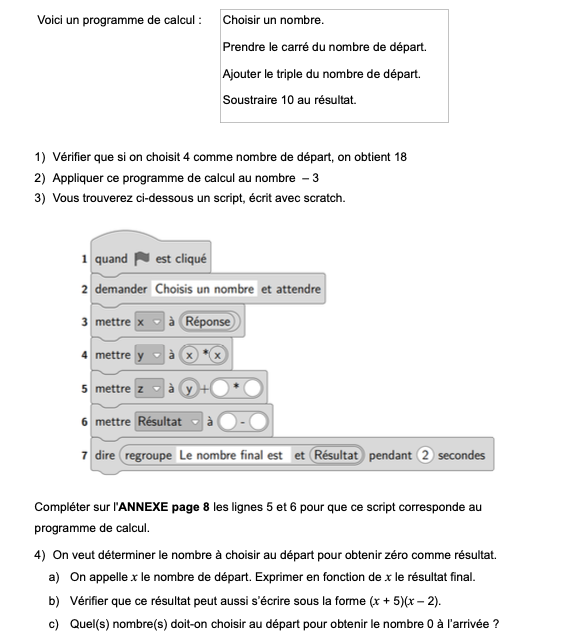
\includegraphics[width = 19 cm]{ex1} 
	 
 	\end{document}







